\section{径迹判选和电子鉴别}
在每个54.4 GeV 金-金对撞的事例中,末态平均可以有几百条径迹被STAR测量到。为了从中更好的挑选出电子径迹来进行最后的分析,一些关于径迹质量和粒子鉴别的判选条件被用来将可能是电子的径迹挑选出来。下面的章节将对这两组判选条件进行详细的介绍。
\subsection{径迹判选}
在本分析中,我们主要用到的探测器是时间投影室和飞行时间探测器。由于探测器本身的限制,我们所用的径迹应该在这两个探测器的接受度范围内而且可以被探测器很好地重建出来。
这样一来,用于在分析中进行电子对重建的电子的径迹应该满足探测器接收度和径迹重建质量上的需求,从而保证分析的质量。

首先对于一条径迹来说,在本分析中希望这条径迹是一条有着足够多的点,即粒子穿过时间投影室时可以在时间投影室当中留下足够多的击中来进行径迹重建。自然而然地在本分析当中就对径迹用来重建的击中数(nHitsFit)有了要求。当两条粒子的轨迹在空间位置上很近的时候,在时间投影室中留下的击中容易被算法识别为同一条径迹留下的击中。为了避免这种情况,对一条径迹用来重建的击中数和最大(nHitsfit/nHitsPoss)的比值应该大于0.52。又因为时间投影室同时可以利用粒子穿过时的电离能损信息来进行粒子鉴别,具体方法在\ref{chap:TPC}当中已经进行过讨论,和重建类似,一条满足径迹质量要求的径迹需要有足够的点来进行能量损失的计算,这也就对径迹用来计算电离能损的击中数(nHitsFit)有了要求。
因为在本分析当中希望分析的电子来自于QGP直接产生或者来自于短寿命介子的衰变的电子,这就要求电子要来自于主碰撞顶点(Primary Vertex)而不是次级的衰变顶点。这就要求径迹到主碰撞顶点的最近距离(distance of closest approach,DCA)小于1cm。

详细的径迹质量判选条件和径迹的接受度范围在表\ref{tab:TrackQuality}左栏中列出。


\begin{table}[h!]
    \centering
    \caption{径迹质量和电子鉴别(eID)判选条件}
    \label{tab:TrackQuality}
    \begin{tabularx}{0.8\textwidth} {
    | >{\centering\arraybackslash}X |>{\centering\arraybackslash}X | }
        \hline
        径迹质量判选 & 电子鉴别(eID)   \\
        \hline
        $0.2 \leq p_{T} \leq 30 GeV/c $ & $p<0.8 GeV/c $ \\
        $|\eta| \leq 1 $ & $ 3*p - 3.15 \leq |n\sigma_{e}| \geq 2.0$  \\
        $dca \leq 1cm $ & $p \geq 0.8 GeV/c $\\ 
        $N_{HitsFit} \geq 20 $  & $ -0.75 \leq |n\sigma_{e}| \geq 2.0 $\\
        ${N_{HitsFit}}/{N_{HitsPoss}} \geq 0.52 $ &  $|1-1/\beta| < 0.25 $\\
        $N_{HitsDedx} \geq 15 $  & \\
        \hline
    \end{tabularx}
\end{table}

\subsection{电子鉴别(eID)}
\label{ch:eID}
经过径迹质量的判选后,所有的径迹再通过电离能损和速度的信息来判断是否为可能的电子候选者。
径迹在通过了径迹质量和接收度的判选之后,通过径迹的电离能损和速度信息就可以辨别出来该径迹是否有可能为一条由电子留下来的径迹。
将每条径迹由时间投影室测量得到的电离能损和通过BB公式计算得到的电子电离能损相比较可以得到一个归一化的值,\nSigmaE ,如式\ref{eq:nSigmaE}所示。在理想情况下,电子的$n\sigma_\mathrm{e}$应该为一个中心值为0的高斯分布。在$P > 1 GeV$时,电子在工作气体中的电离能损和其他粒子重合,无法单纯的通过电离能损鉴别粒子。这时可以将电离能损和TOF测得的速度信息结合来进行离子鉴别。因为电子质量轻于其它强子,在相同动量下粒子的速度会大于其他粒子,所以可以额外添加一个$1/\beta$的判选条件来进行电子鉴别。电子鉴别的条件在表\ref{tab:TrackQuality}的右栏列出。图 a,b分别为$n\sigma_\mathrm{e}$的分布和加上$1/\beta$判选条件后的$n\sigma_\mathrm{e}$分布。

\begin{equation}
    \label{eq:nSigmaE}
    n\sigma_e = \frac{log(\frac{dE/dx_{measure}}{dE/dx_{BB}})}{\sigma_{dE/dx}}
\end{equation}

\begin{figure}[htb]
    \centering
    \begin{subfigure}[b]{0.45\textwidth}
        \centering
        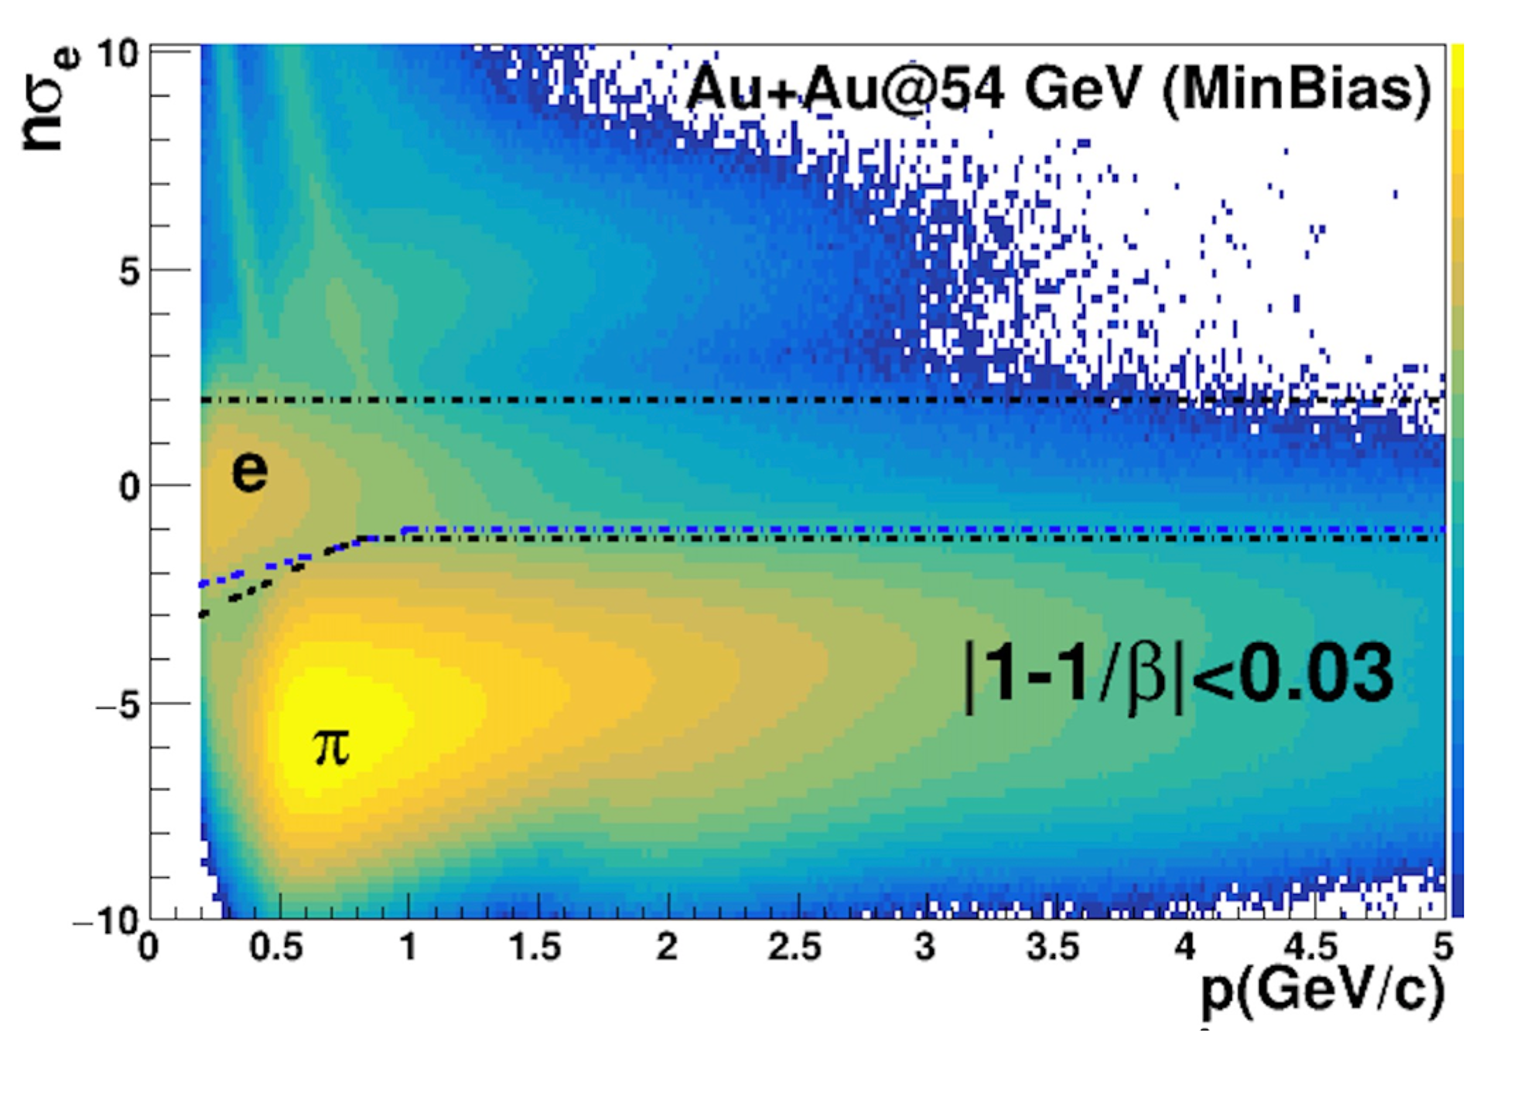
\includegraphics[width=\textwidth,clip]{figures/Chapter4/nSigmaEwTOF.png}
        \caption{}
        \label{fig:nSigmaEwTOF}
    \end{subfigure}
    \hfill
    \begin{subfigure}[b]{0.49\textwidth}
        \centering
        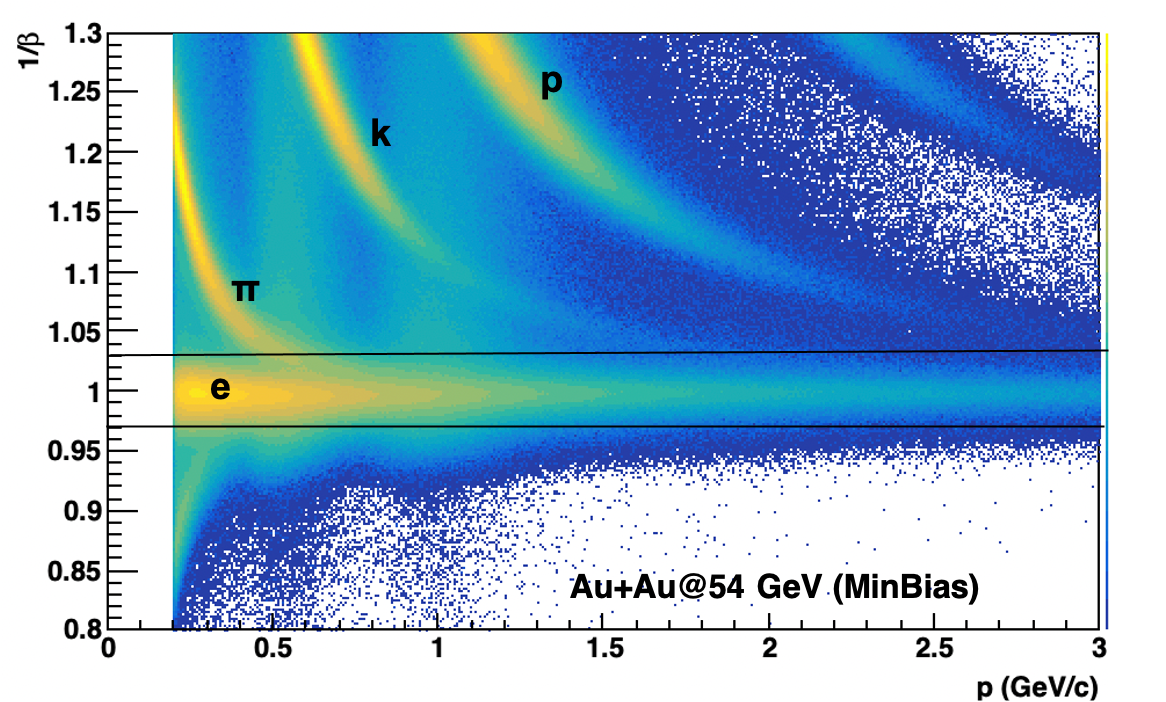
\includegraphics[width=\textwidth,clip]{figures/Chapter4/beta_Cut.png}
        \caption{}
        \label{fig:beta_Cut}
    \end{subfigure}
       \caption[\nSigmaE 和 $1/\beta$判选条件示意图]{图\ref{fig:nSigmaEwTOF}为\nSigmaE 判选条件示意图,其中黑色虚线为\sNN = 54.4GeV 中 \nSigmaE 的判选条件上下限。图 \ref{fig:beta_Cut} 为$1/\beta$判选条件示意图, 黑色实线为判选条件上下限 }
       \label{fig:eID_cut}
\end{figure}